\begin{figure}
\begin{center}
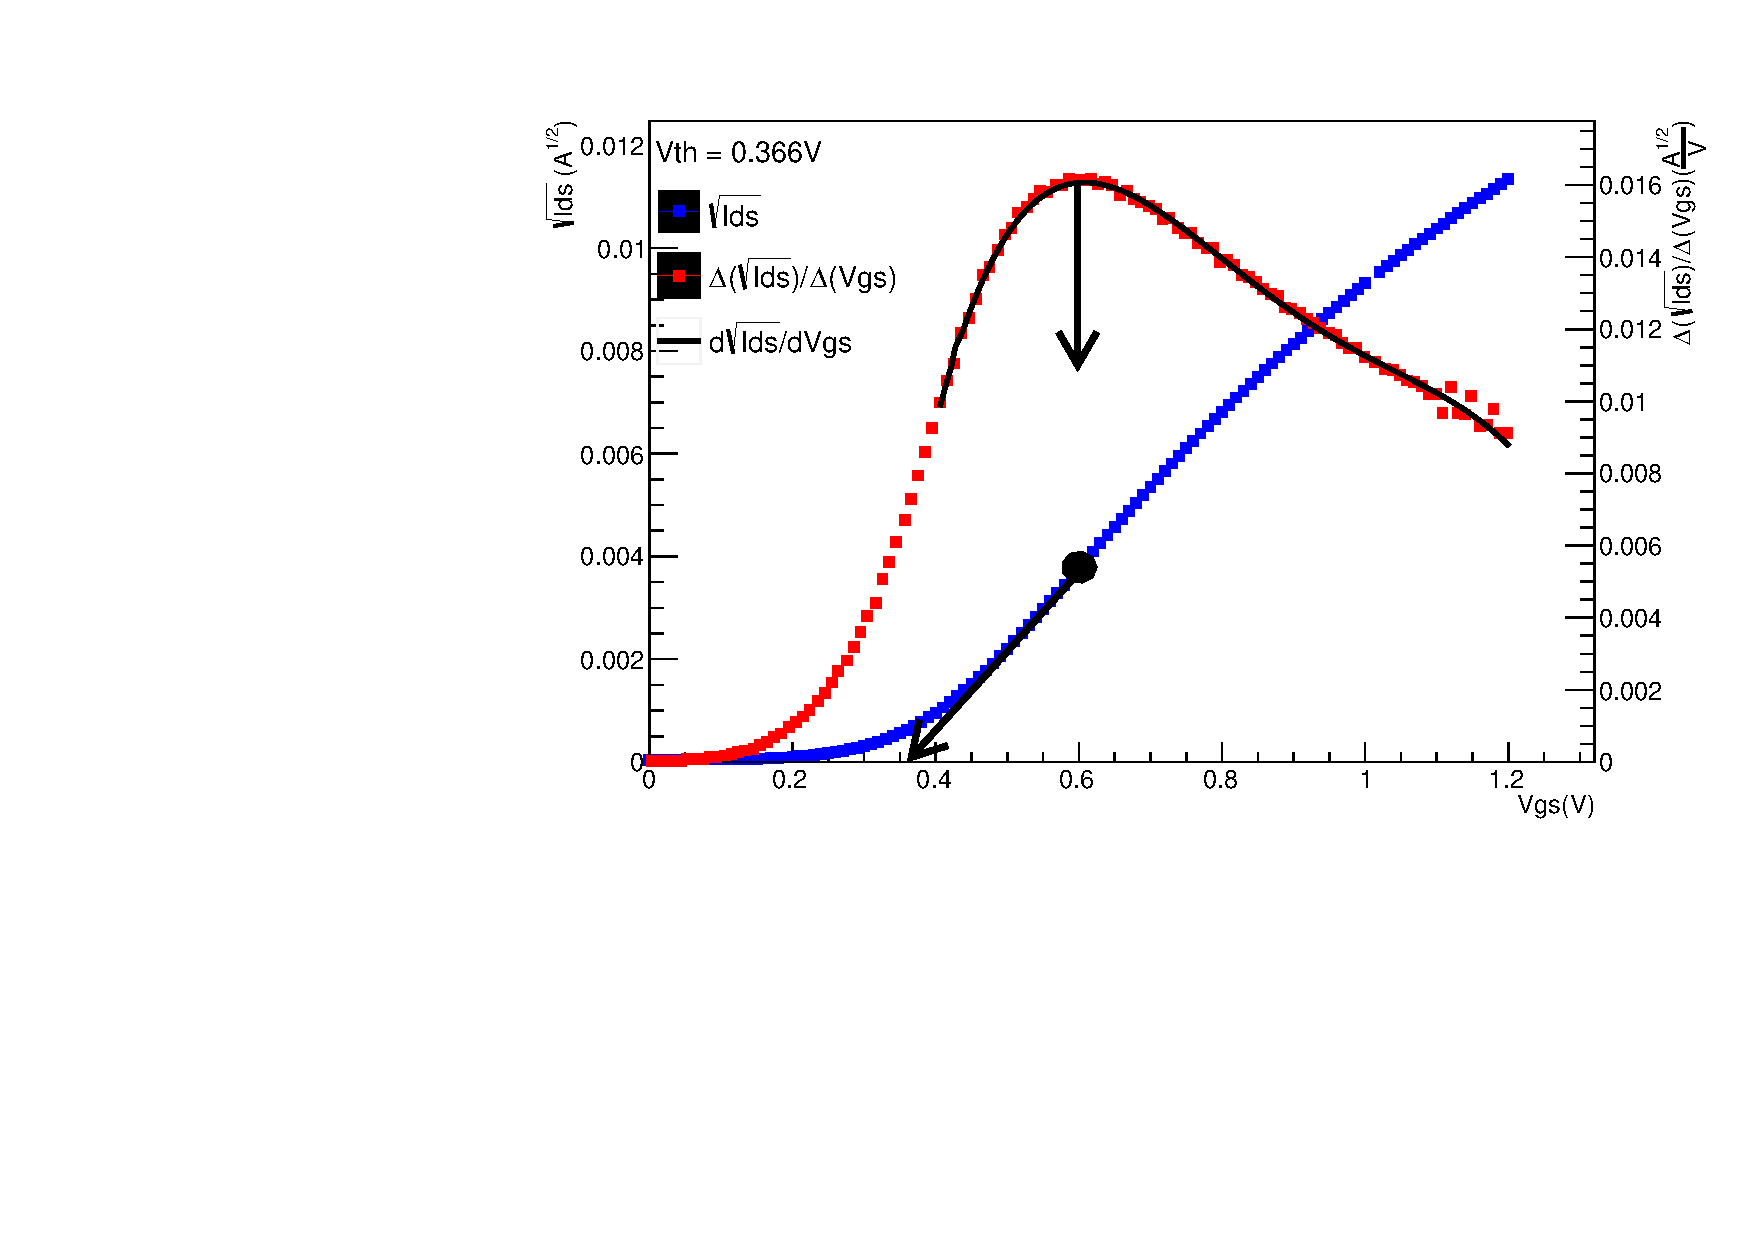
\includegraphics[height=7.12cm]{Quadratic_Method.pdf}
\caption{This figure illustrates the quadratic extrapolation method used to determine the (saturation) threshold voltage ($V_{th}$) of an NMOS transistor.  The data shown is from the pre-irradiation measurement of the 240/60 transistor in IC3.
For PMOS transistors, $|I_{ds}|$ is used since $I_{ds}$ is negative.}
\label{fig:QuadMethod}
\end{center}
\end{figure}

Two quantities were extracted from each transistor characteristic: the maximum drain-source current and the (saturation) threshold voltage $V_{th}$.  The quadratic extrapolation method was used to determine the threshold voltage\cite{Schroder}.  As shown in Figure~\ref{fig:QuadMethod}, $V_{th}$ is defined to be the voltage at which a line tangent to the curve $\sqrt{|I_{ds}|}$ vs $ V_{gs}$ at the point of maximum $\frac{d\sqrt{|I_{ds}|}}{dV_{gs}}$ intercepts the $I_{ds}=0$ axis.  We determined the slope of the curve by fitting it with a fifth order polynomial and differentiating the fit function.  In Figure~\ref{fig:QuadMethod}, the red squares were computed using finite differences
\Big({${\sqrt{I_{ds}(N+1)}-\sqrt{I_{ds}(N)}\over{V_{gs}(N+1)-V_{gs}(N)}}$} \Big); the black line is the result of differentiating the fit to the curve $\sqrt{|I_{ds}|}$ vs $ V_{gs}$.

\begin{figure}
	\begin{minipage}[b]{.5\linewidth}
	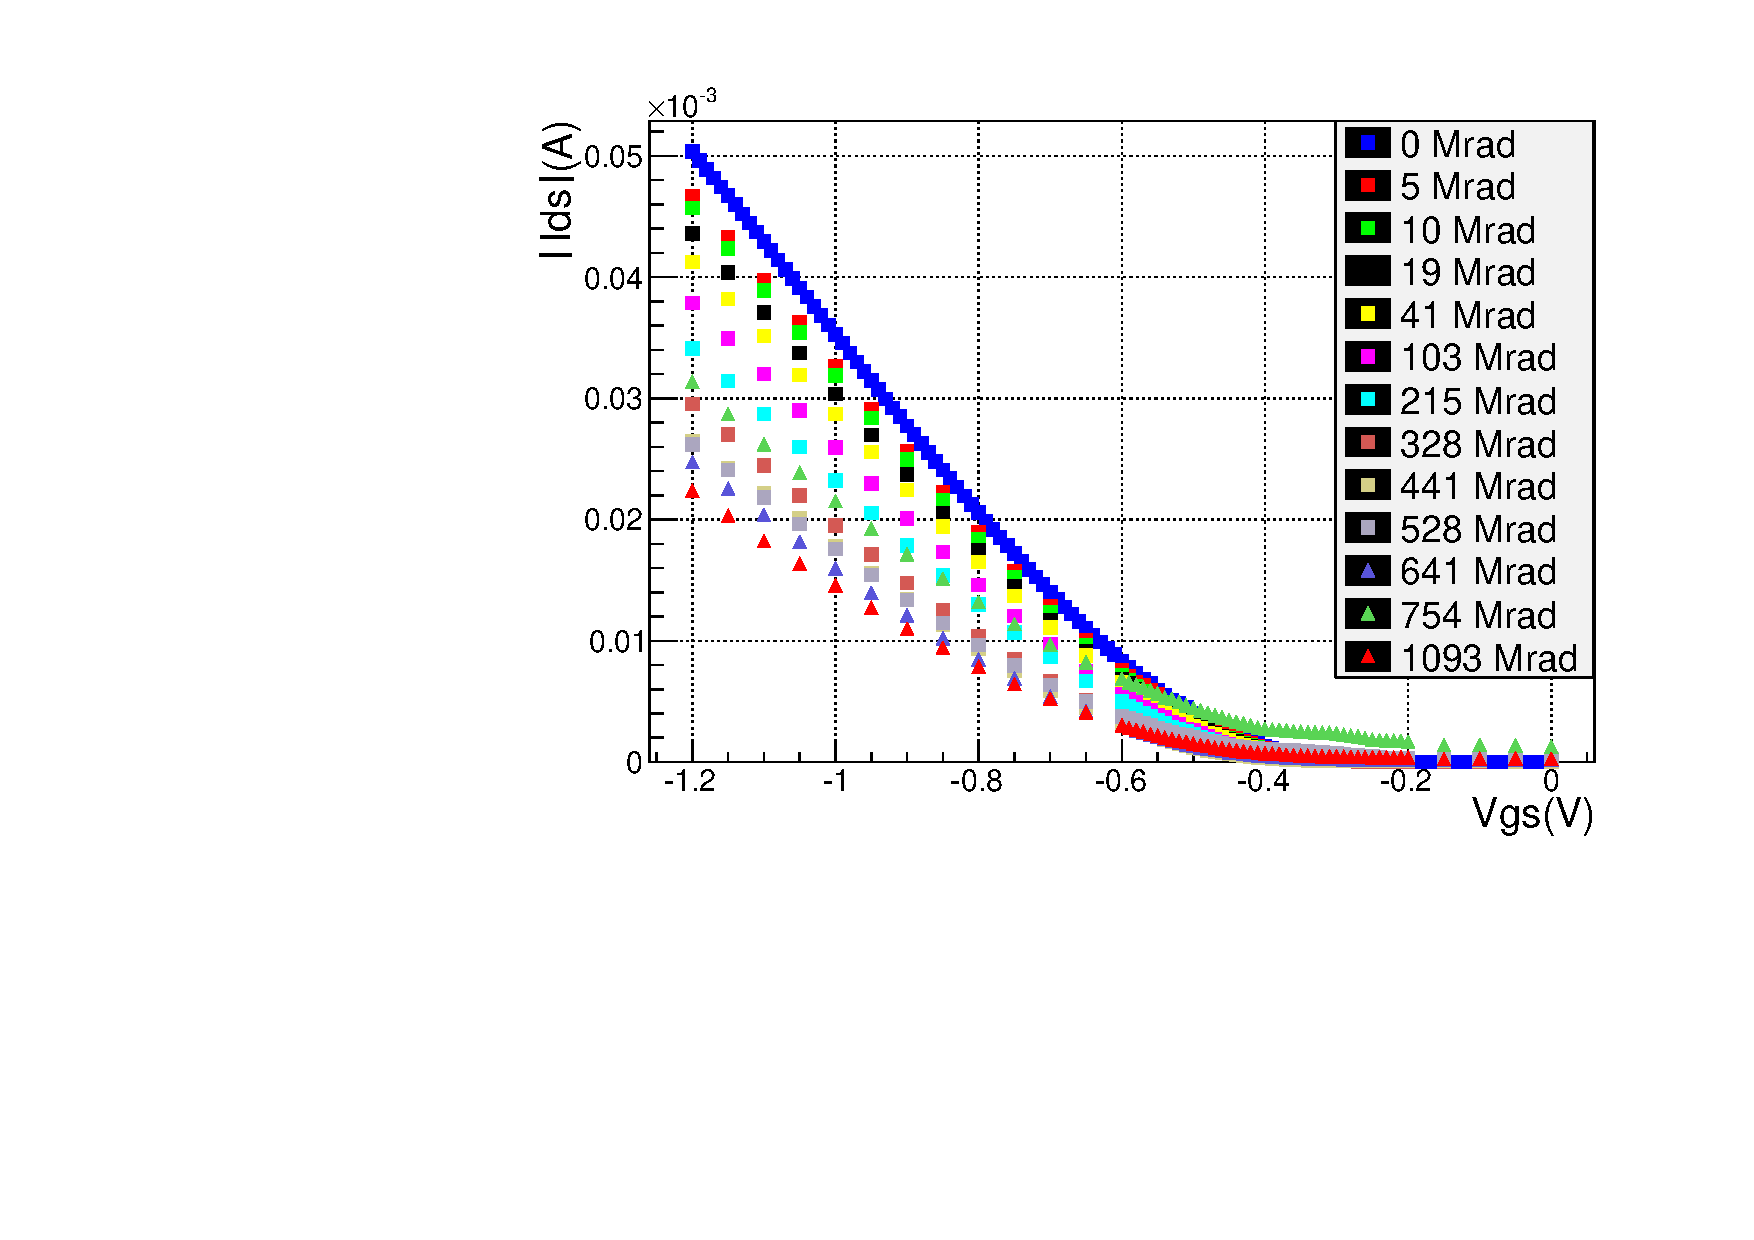
\includegraphics[width=\linewidth]{pd012_2_comparison_paper.pdf}
	\end{minipage}
	\begin{minipage}[b]{.5\linewidth}
	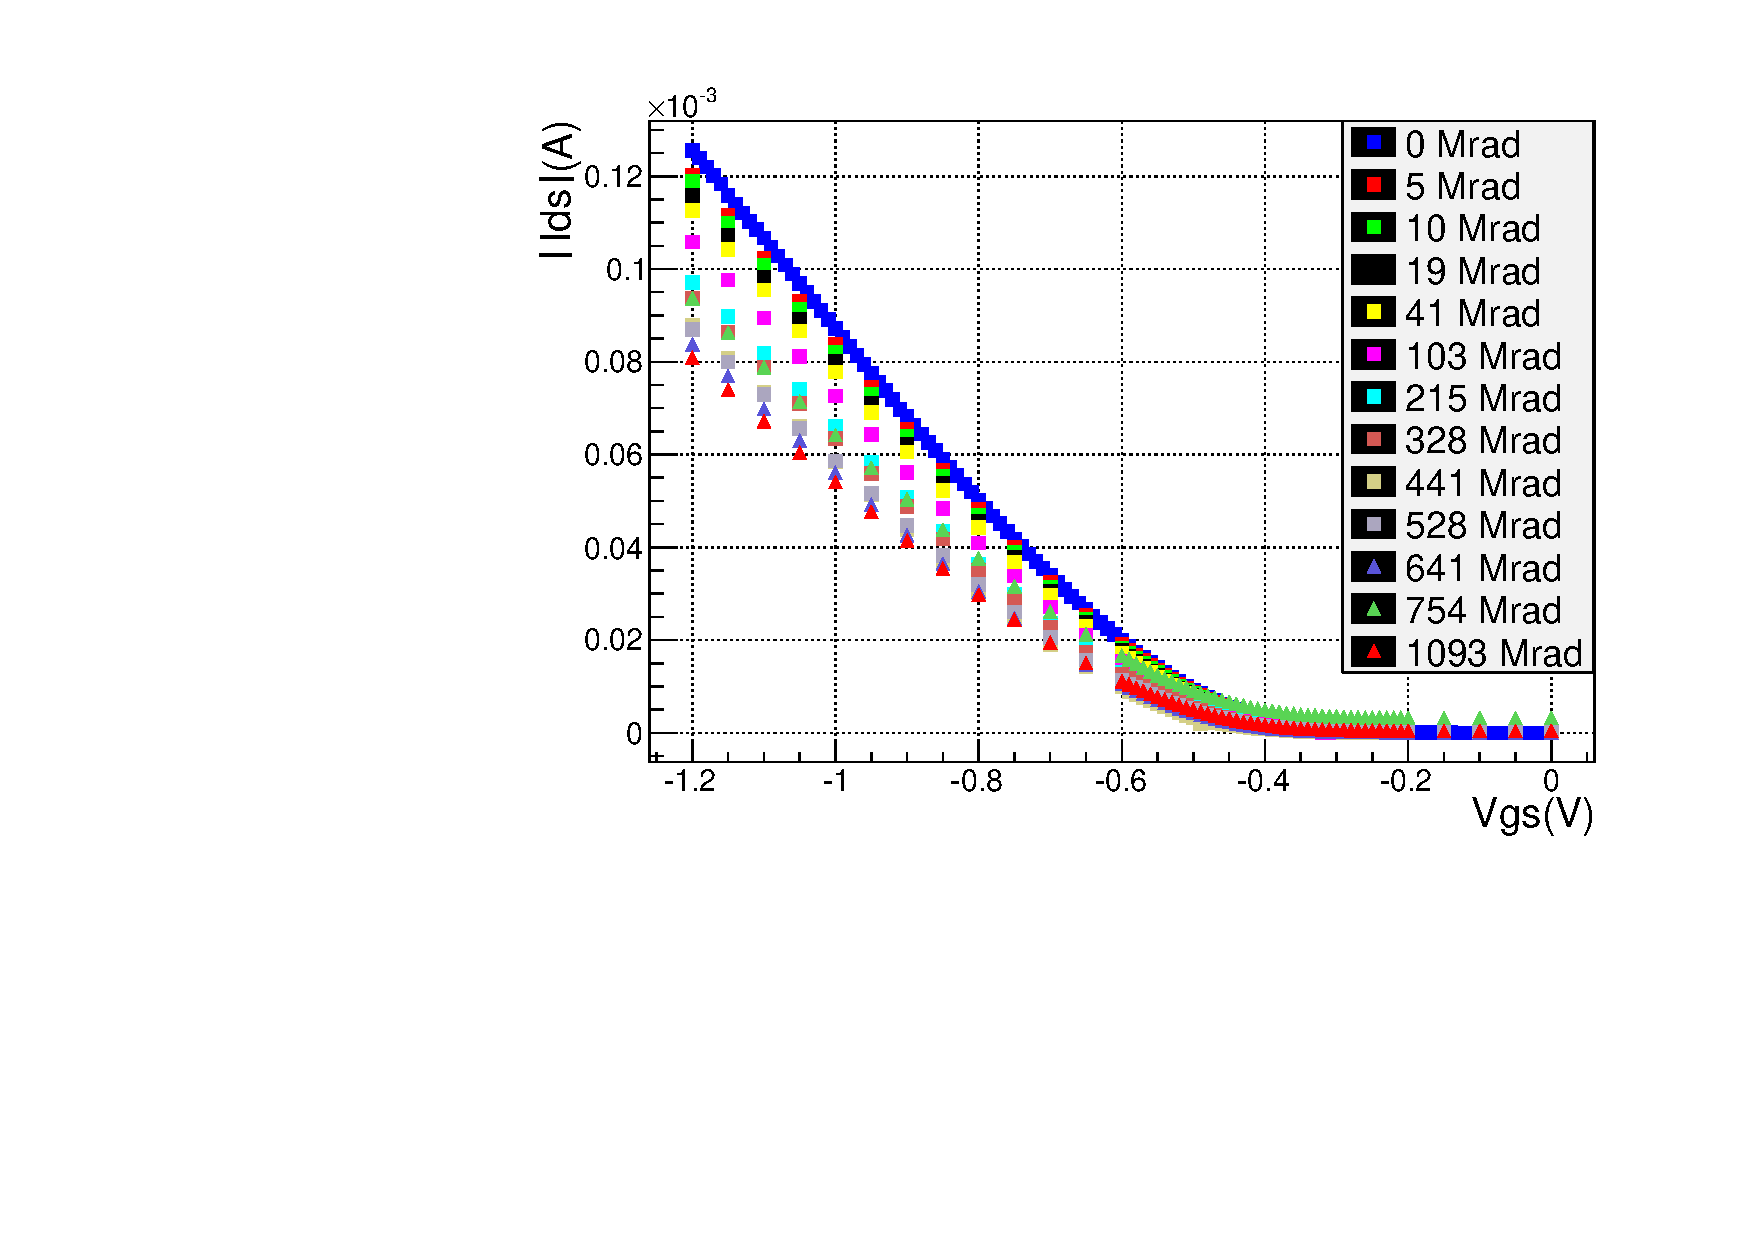
\includegraphics[width=\linewidth]{pd036_2_comparison_paper.pdf}
	\end{minipage}
	\begin{minipage}[b]{.5\linewidth}
	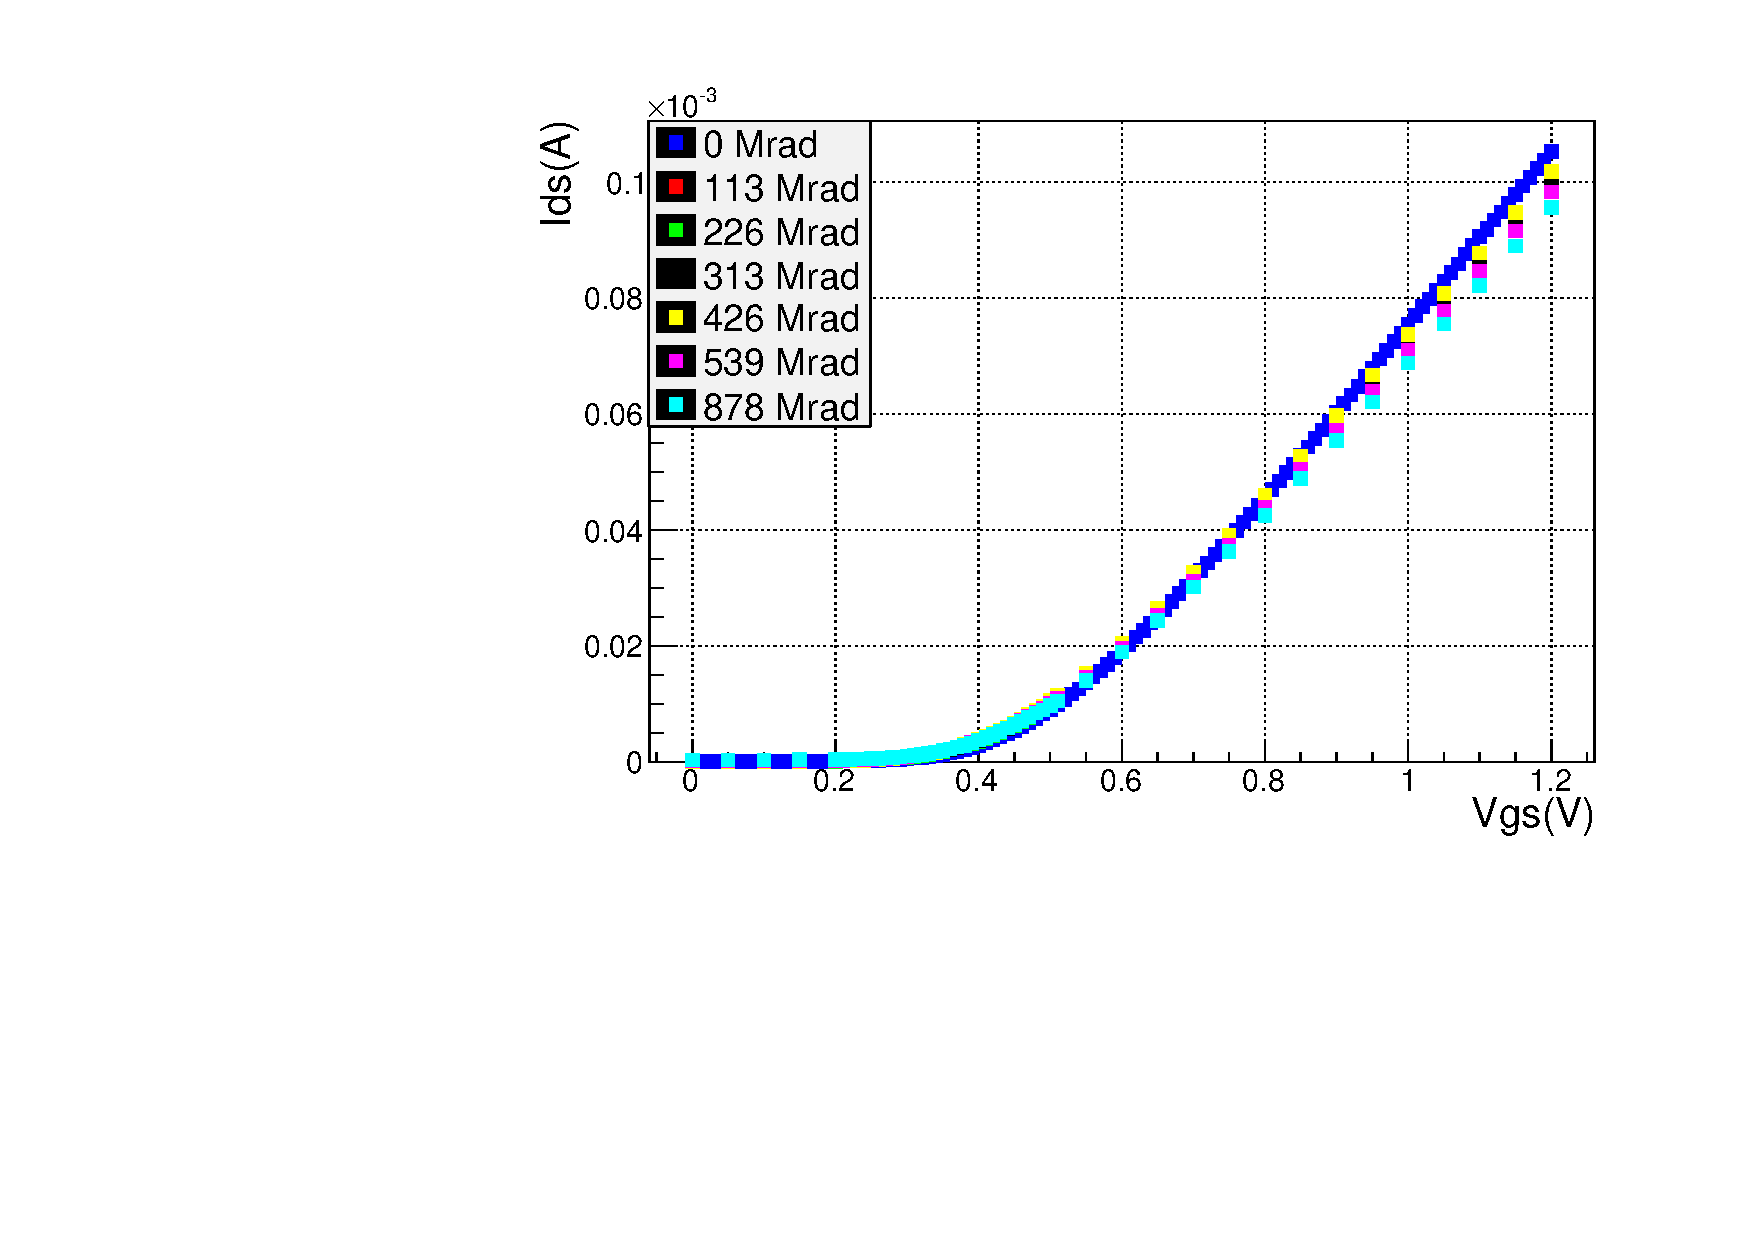
\includegraphics[width=1\linewidth]{d024_1_comparison_paper.pdf}
	\end{minipage}
	\hfill
	\begin{minipage}[b]{.5\linewidth}
	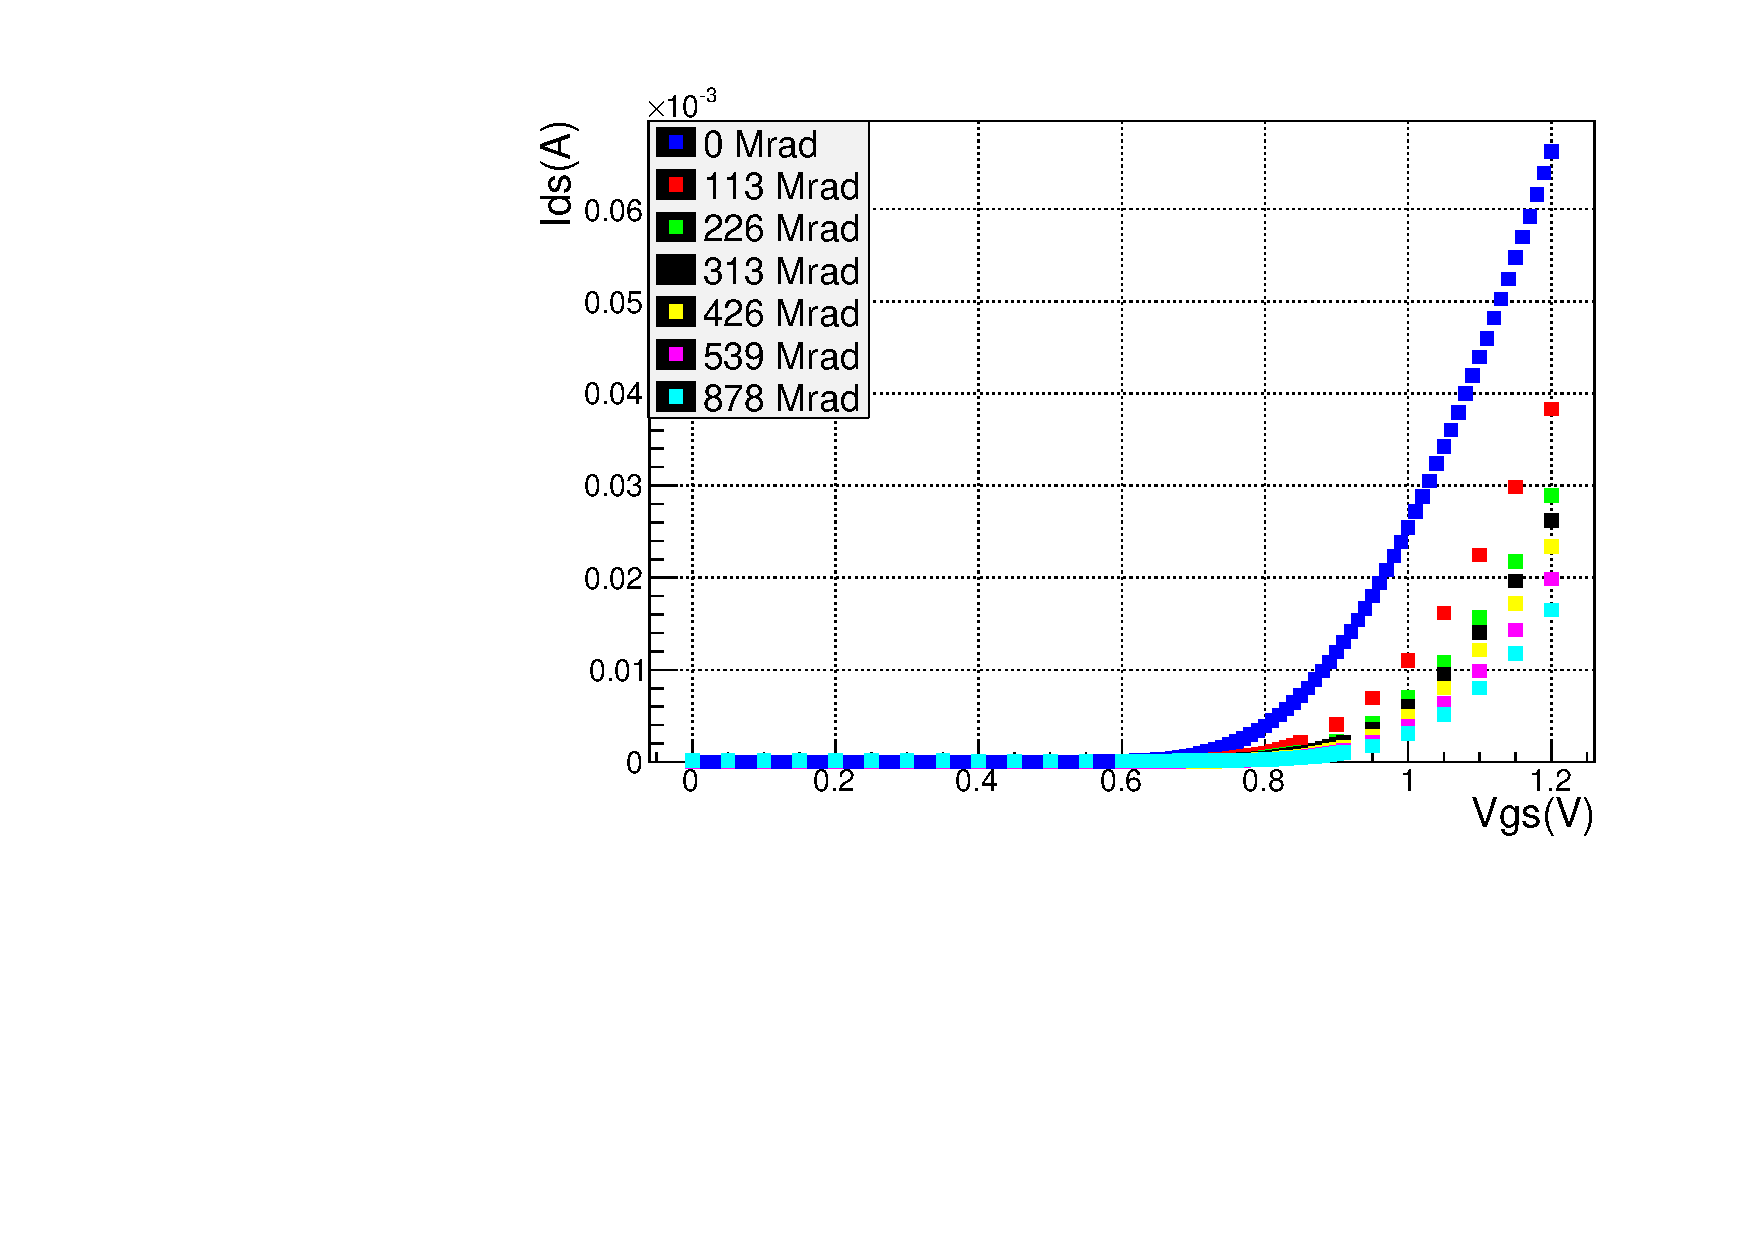
\includegraphics[width=\linewidth]{ddg1u_1_comparison_paper.pdf}
	\end{minipage}
\caption{Transistor characteristic curves for total dose up to 1.1 Grad of (upper left) a 120/60 core PMOS, (upper right) a 360/60 core PMOS, and for total dose up to 878 Mrad of (lower left) a 240/60 core NMOS, and (lower right) a 1000/280 2.5 V NMOS.}
\label{fig:SuperpositionPlots}
\end{figure}

Figure~\ref{fig:SuperpositionPlots} illustrates the radiation effects observed in our data.  The most prominent effect is a decrease of the maximum drain-source current of core PMOS transistors.  The fractional decrease is largest for the smallest PMOS transistors; the maximum drain-source current of the smallest PMOS decreased by more than a factor of two.  The maximum drain-source current of core NMOS transistors also decreased, but only by $\sim5-10\%$.  No significant threshold shift was observed for any of the core transistors, but the threshold voltage of NMOS I/O transistors increased by 100 - 200 mV.  No error bars are included in the figures because the uncertainty in the SMU measurements is smaller than the symbols used to plot the measurements.

\begin{figure}
\begin{minipage}[b]{0.5\textwidth}
	\centering
	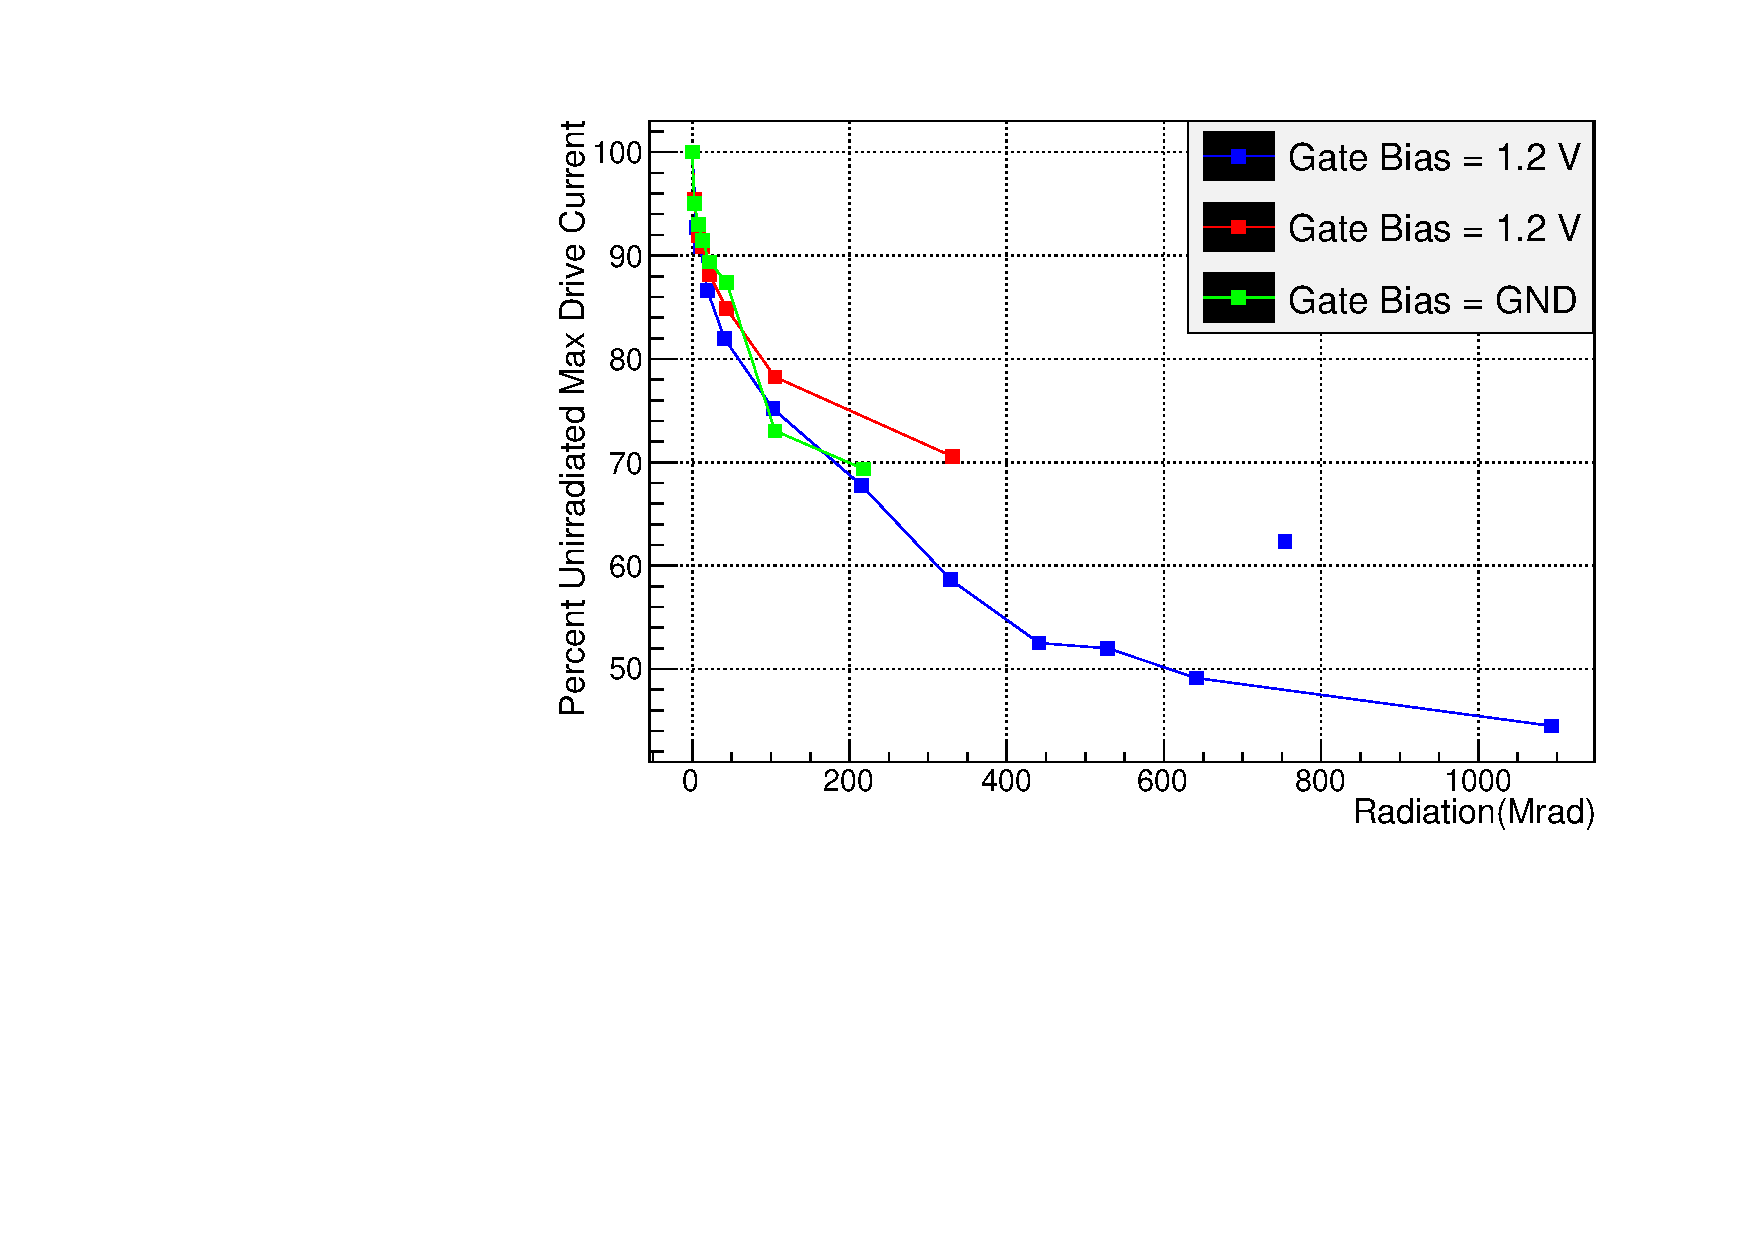
\includegraphics[width=\linewidth]{pd012_comparing_bias_conditions_paper.pdf}
\end{minipage}
\hspace{0.5cm}
\begin{minipage}[b]{0.5\textwidth}
	\centering
	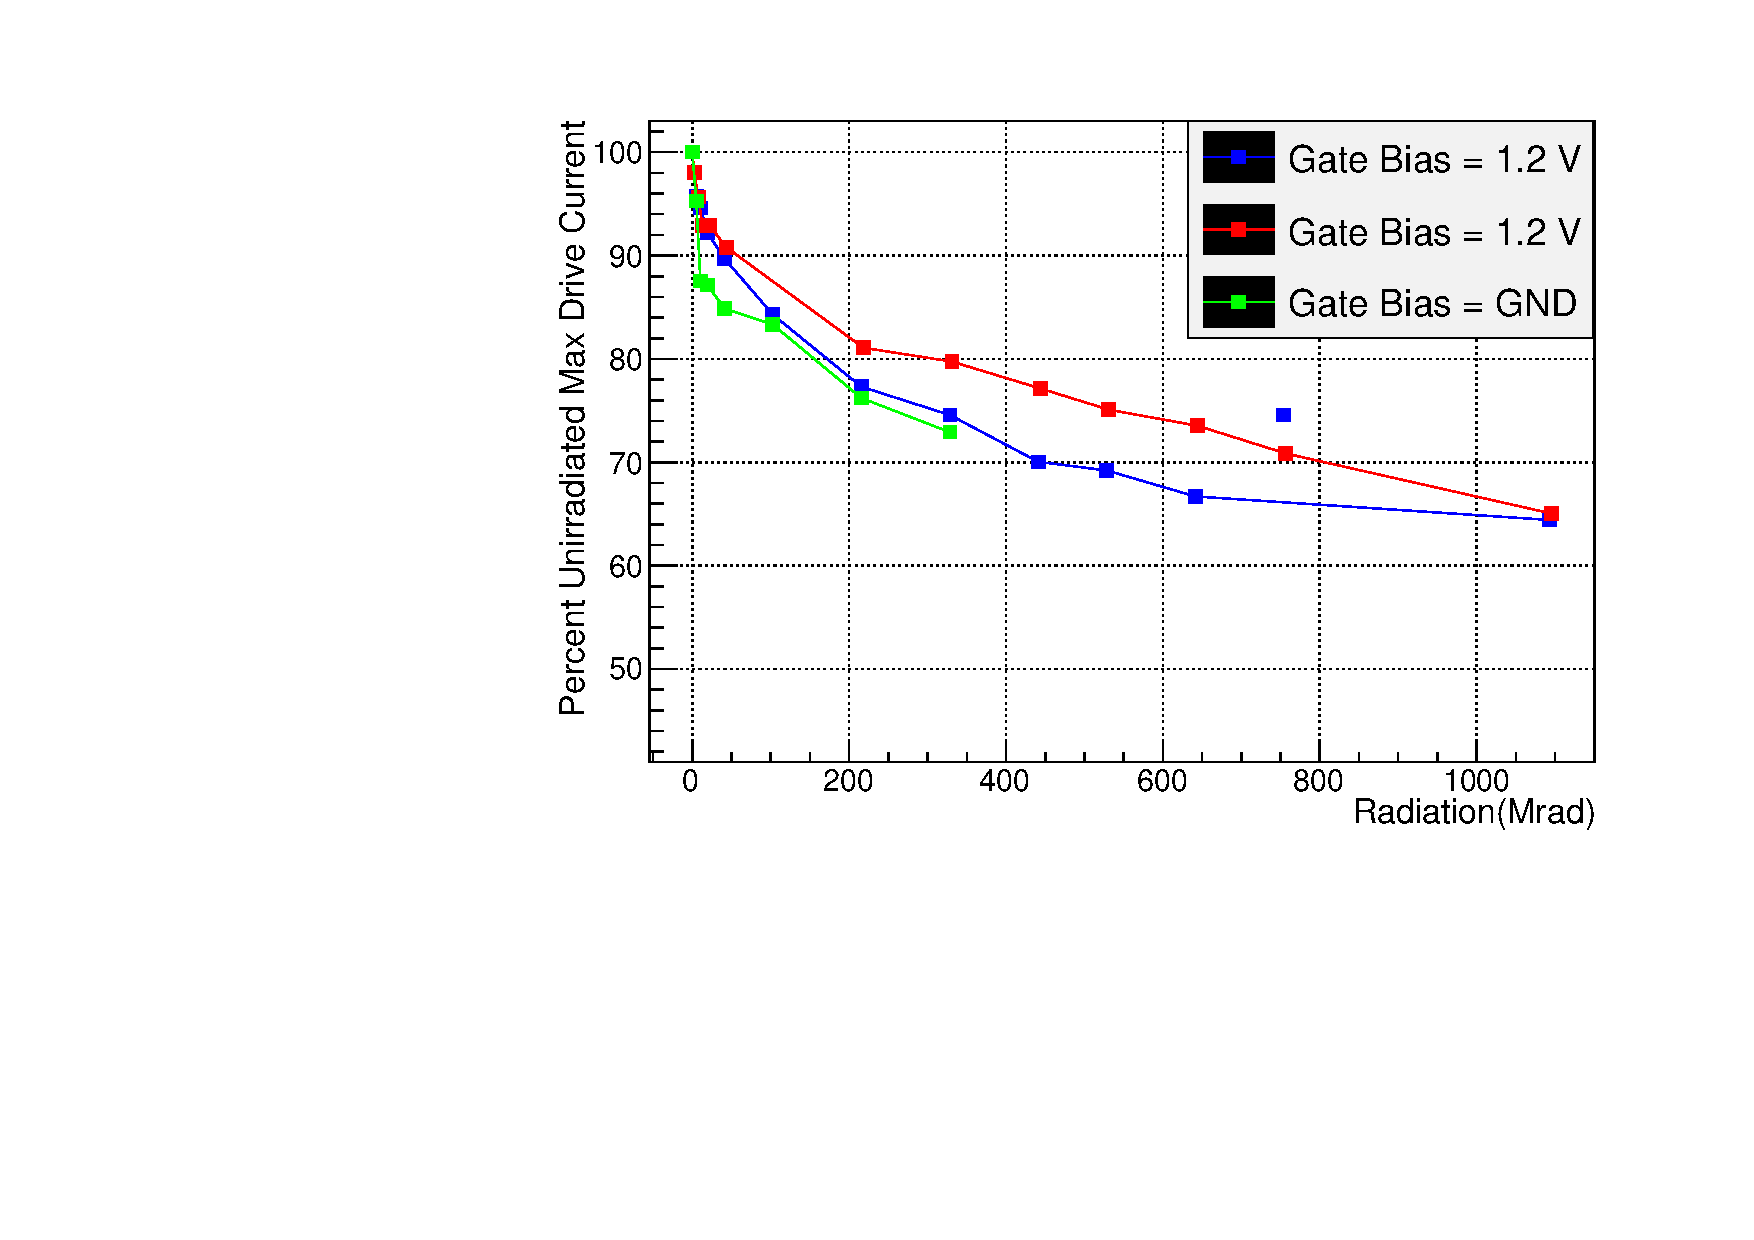
\includegraphics[width=\linewidth]{pd036_comparing_bias_conditions_paper.pdf}
\end{minipage}
\caption{The change in maximum drain-source current for similar PMOS core transistors irradiated with different gate bias voltages. The graph on the left is for 120/60 transistors and the graph on the right is for 360/60 transistors.  The lines connecting points do not represent a fit, and are included only to make the plots easier to read.  The transistor characteristics measured for transistors in package IC5 after 754 Mrad was accumulated were all offset by current not likely to have passed through the transistors (this can be seen in Figure 5).  Lines are not drawn through these points.  The most likely source of these offsets is leakage current due to moisture caused by condensation on the cold IC package.}
\label{fig:PMOSBiasConditions}
\end{figure}

%No significant difference was observed between the radiation-induced changes of PMOS transistors biased during the irradiation with the gate in the ON state and PMOS transistors biased with the gate in the OFF state.  This is illustrated in Figure~\ref{fig:PMOSBiasConditions}.  We also did not observe any significant differences in the effect of radiation on the various different types of NMOS transistors tested (normal layout, enclosed layout, triple well, and zero $V_{th}$). 

\begin{figure}
\begin{minipage}[b]{0.5\textwidth}
	\centering
	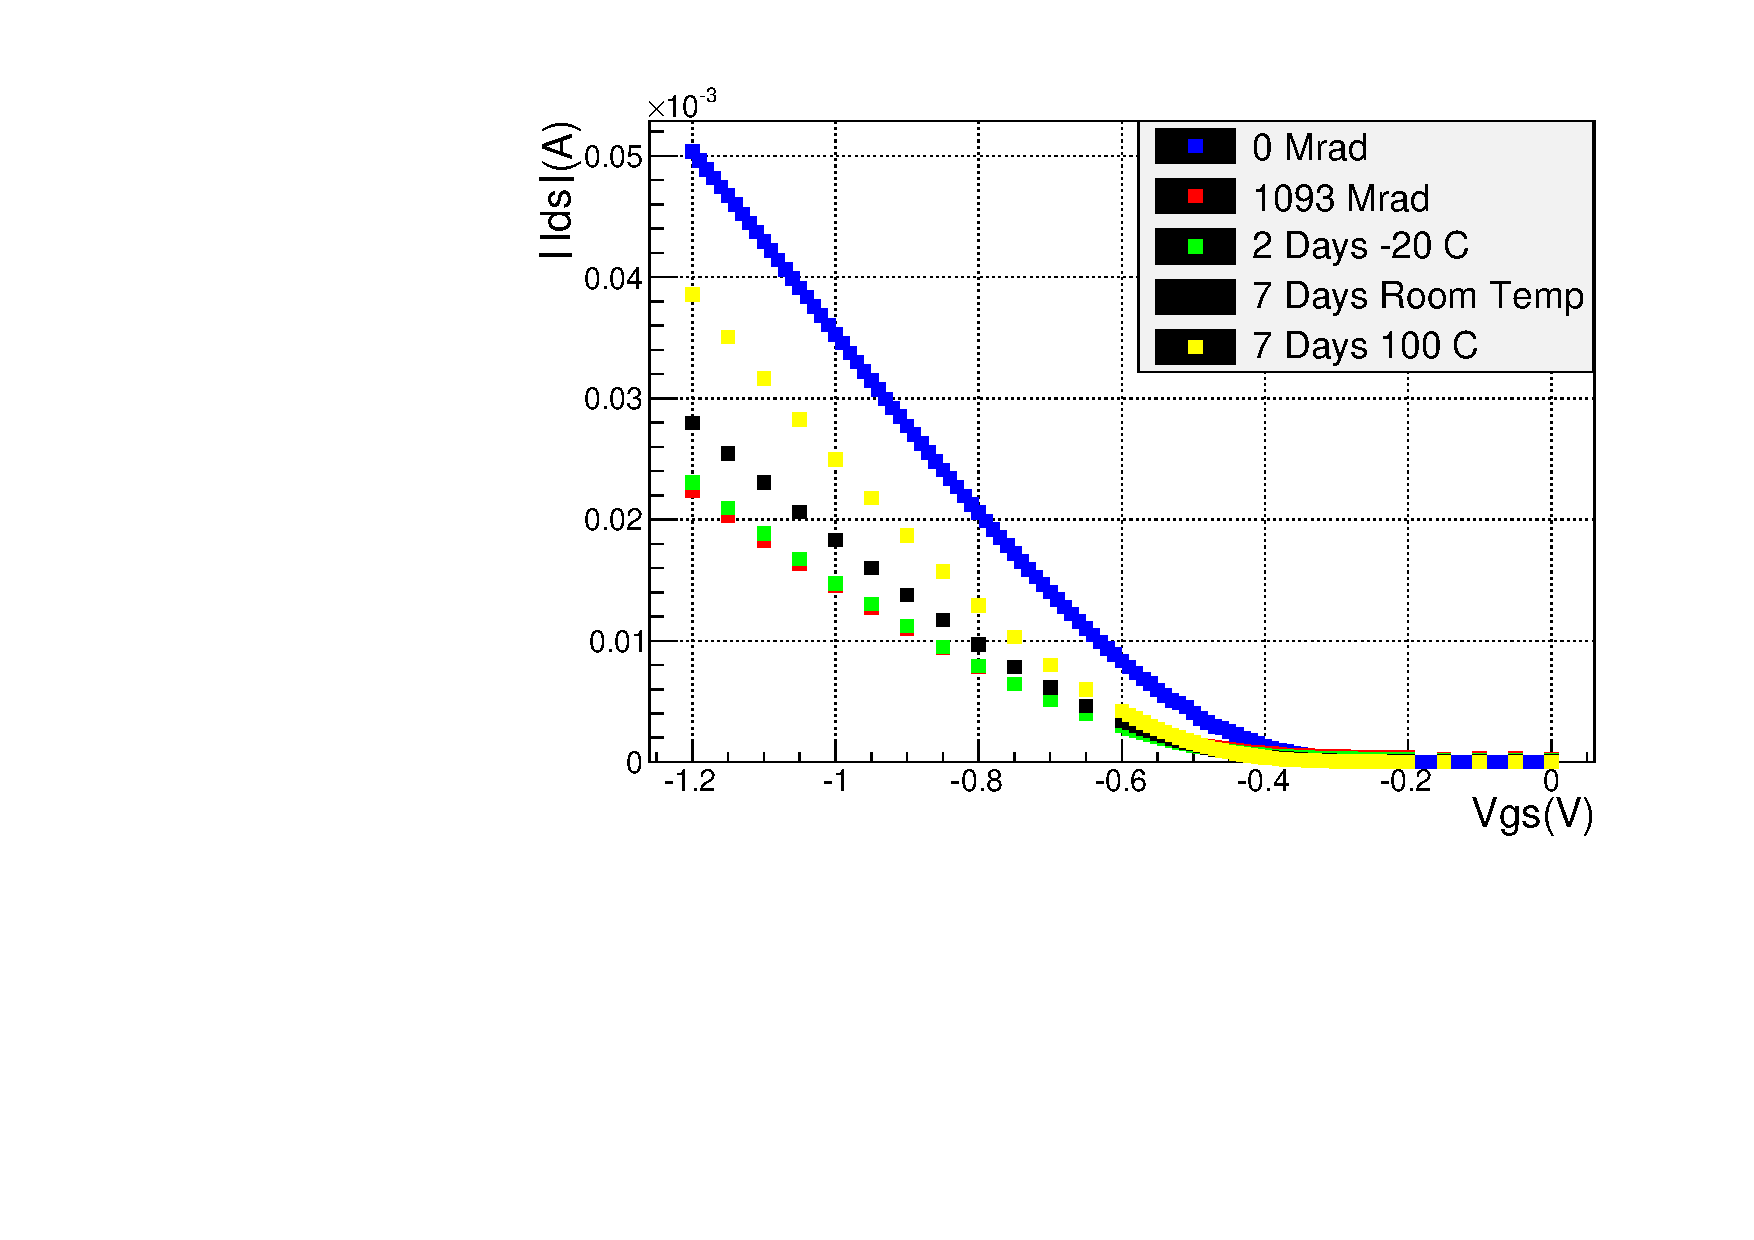
\includegraphics[width=\linewidth]{pd012_2_Anneal_comparison_paper.pdf}
\end{minipage}
\hspace{0.5cm}
\begin{minipage}[b]{0.5\textwidth}
	\centering
	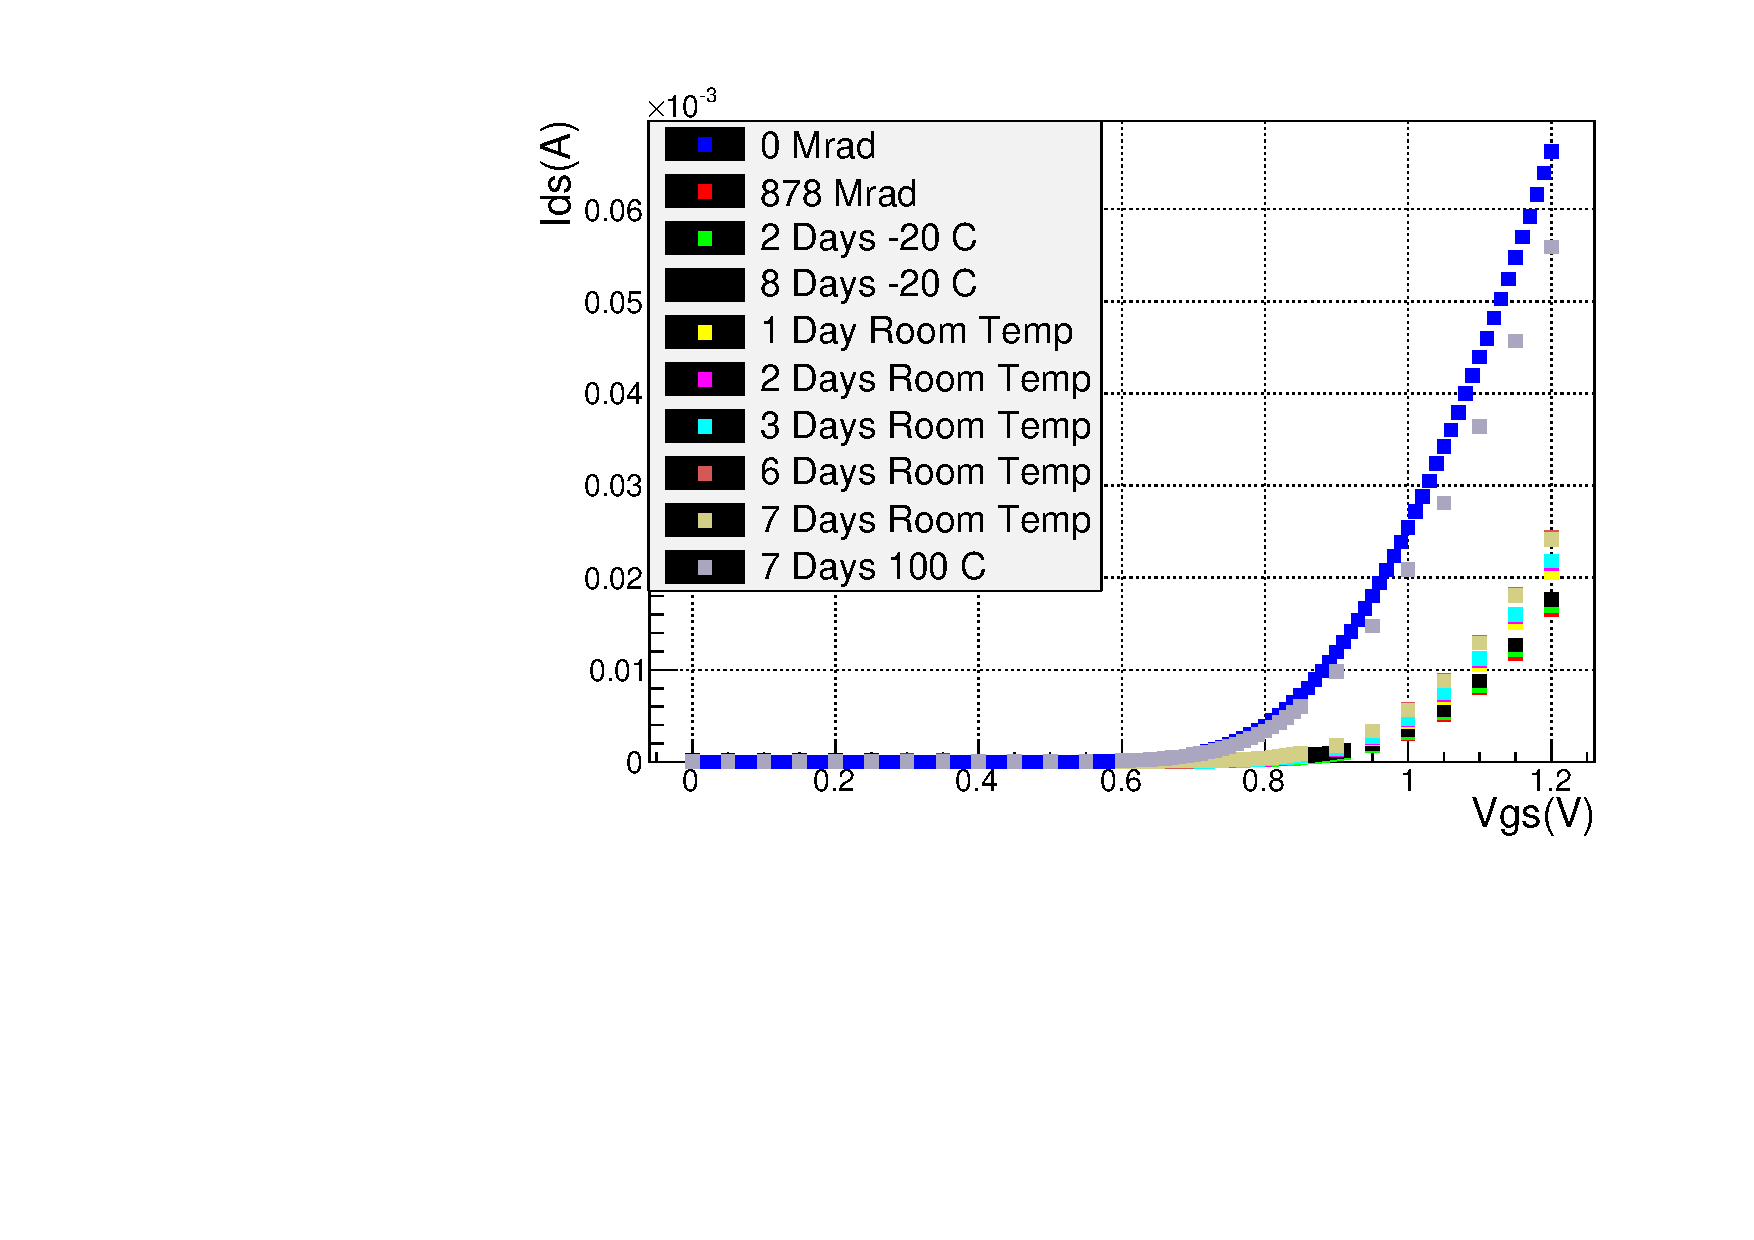
\includegraphics[width=\linewidth]{ddg1u_1_Anneal_comparison_paper.pdf}
\end{minipage}
\caption{Transistor chararcteristic curves during the annealing period for (left) a 120/60 core PMOS and (right) a 1000/280 2.5 V NMOS.}
\label{fig:AnnealSuperpositionPlots}
\end{figure}

No significant difference was observed between the radiation-induced changes of PMOS transistors biased during the irradiation with the gate in the ON state and PMOS transistors biased with the gate in the OFF state.  This is illustrated in Figure~\ref{fig:PMOSBiasConditions}.
%We also did not observe any significant differences in the effect of radiation on the various different types of NMOS transistors tested (normal layout, enclosed layout, triple well, and zero $V_{th}$). 
%Figure~\ref{fig:AnnealSuperpositionPlots} demonstrates the annealing effects observed in our data. Both the PMOS core transistors and the NMOS I/O transistors recovered significantly during the annealing period. 

\begin{figure}
\begin{minipage}[b]{0.5\textwidth}
	\centering
	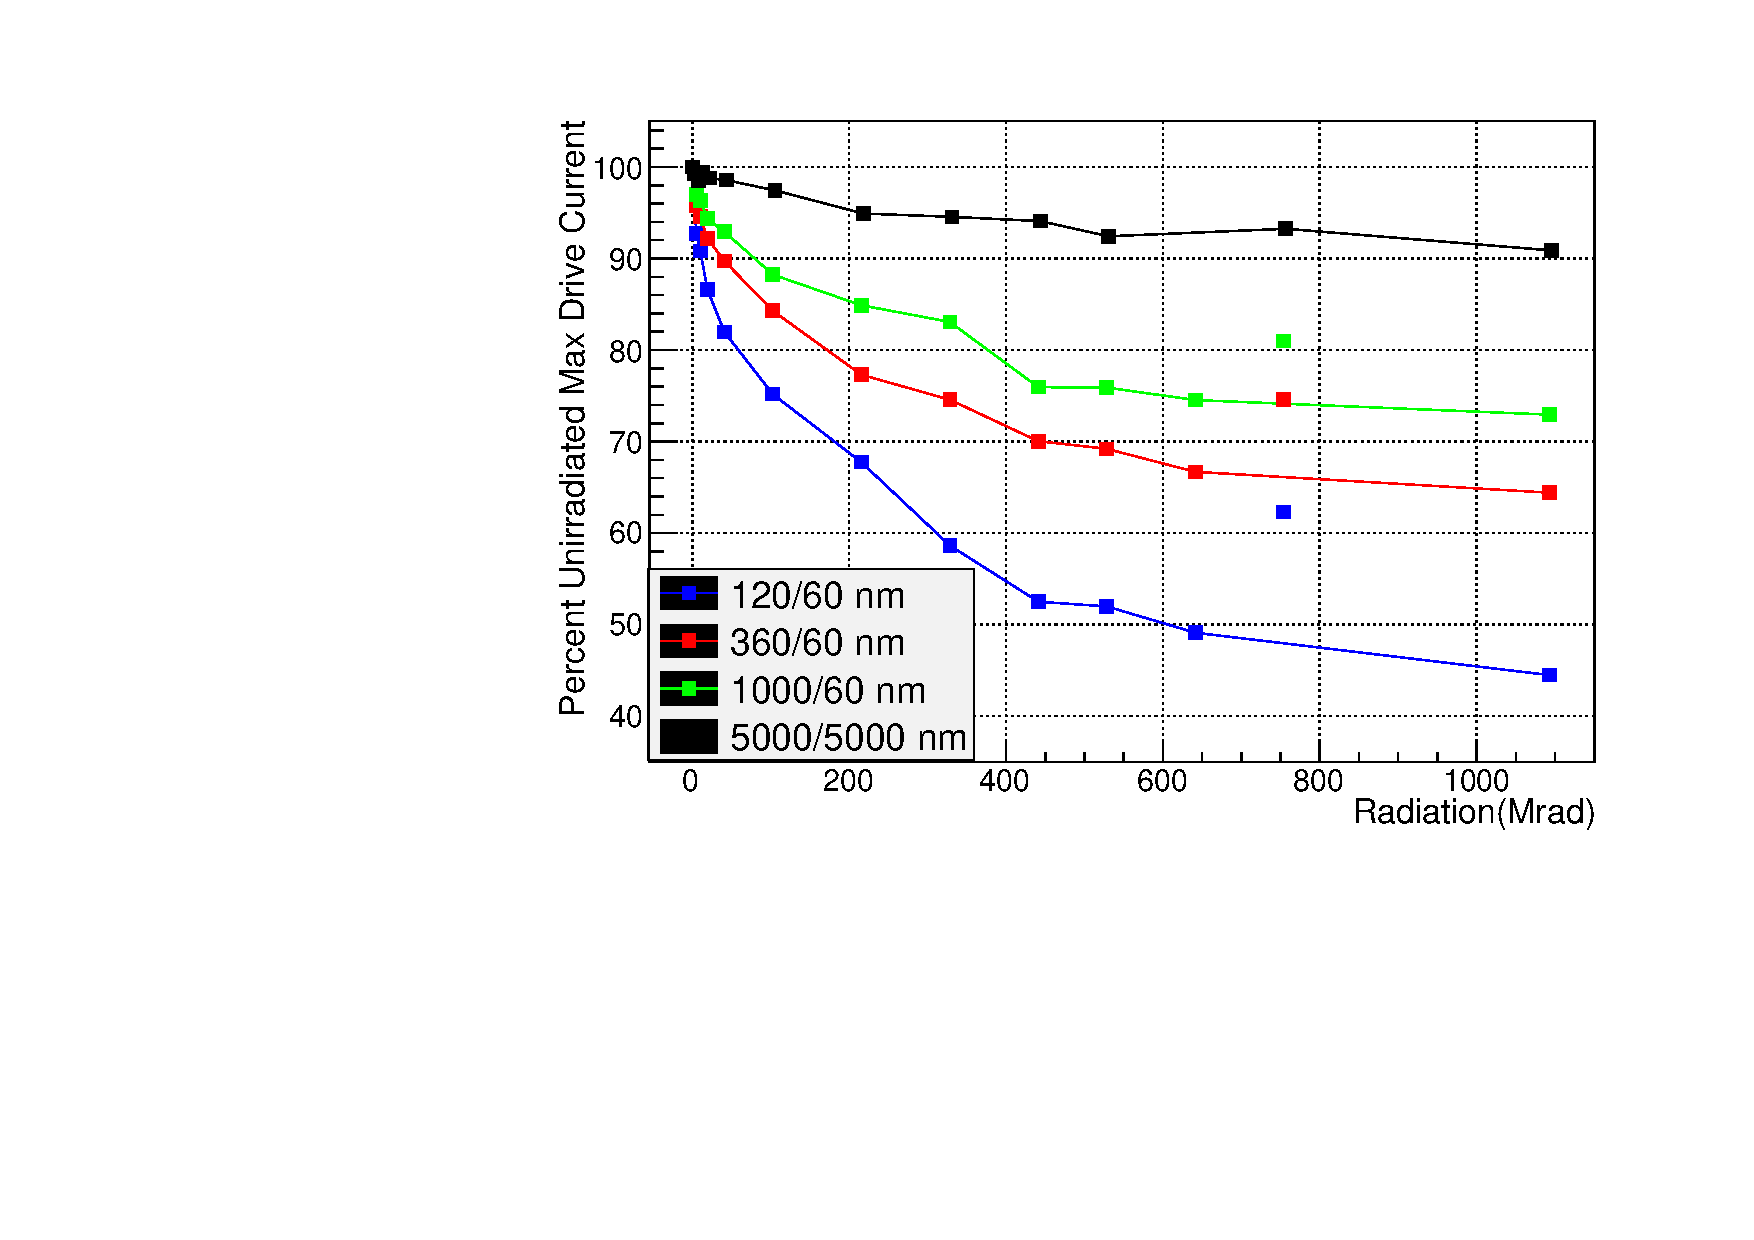
\includegraphics[width=\linewidth]{Comparing_MaxCurrentDrive_PMOS_paper.pdf}
\end{minipage}
\hspace{0.5cm}
\begin{minipage}[b]{0.5\textwidth}
	\centering
	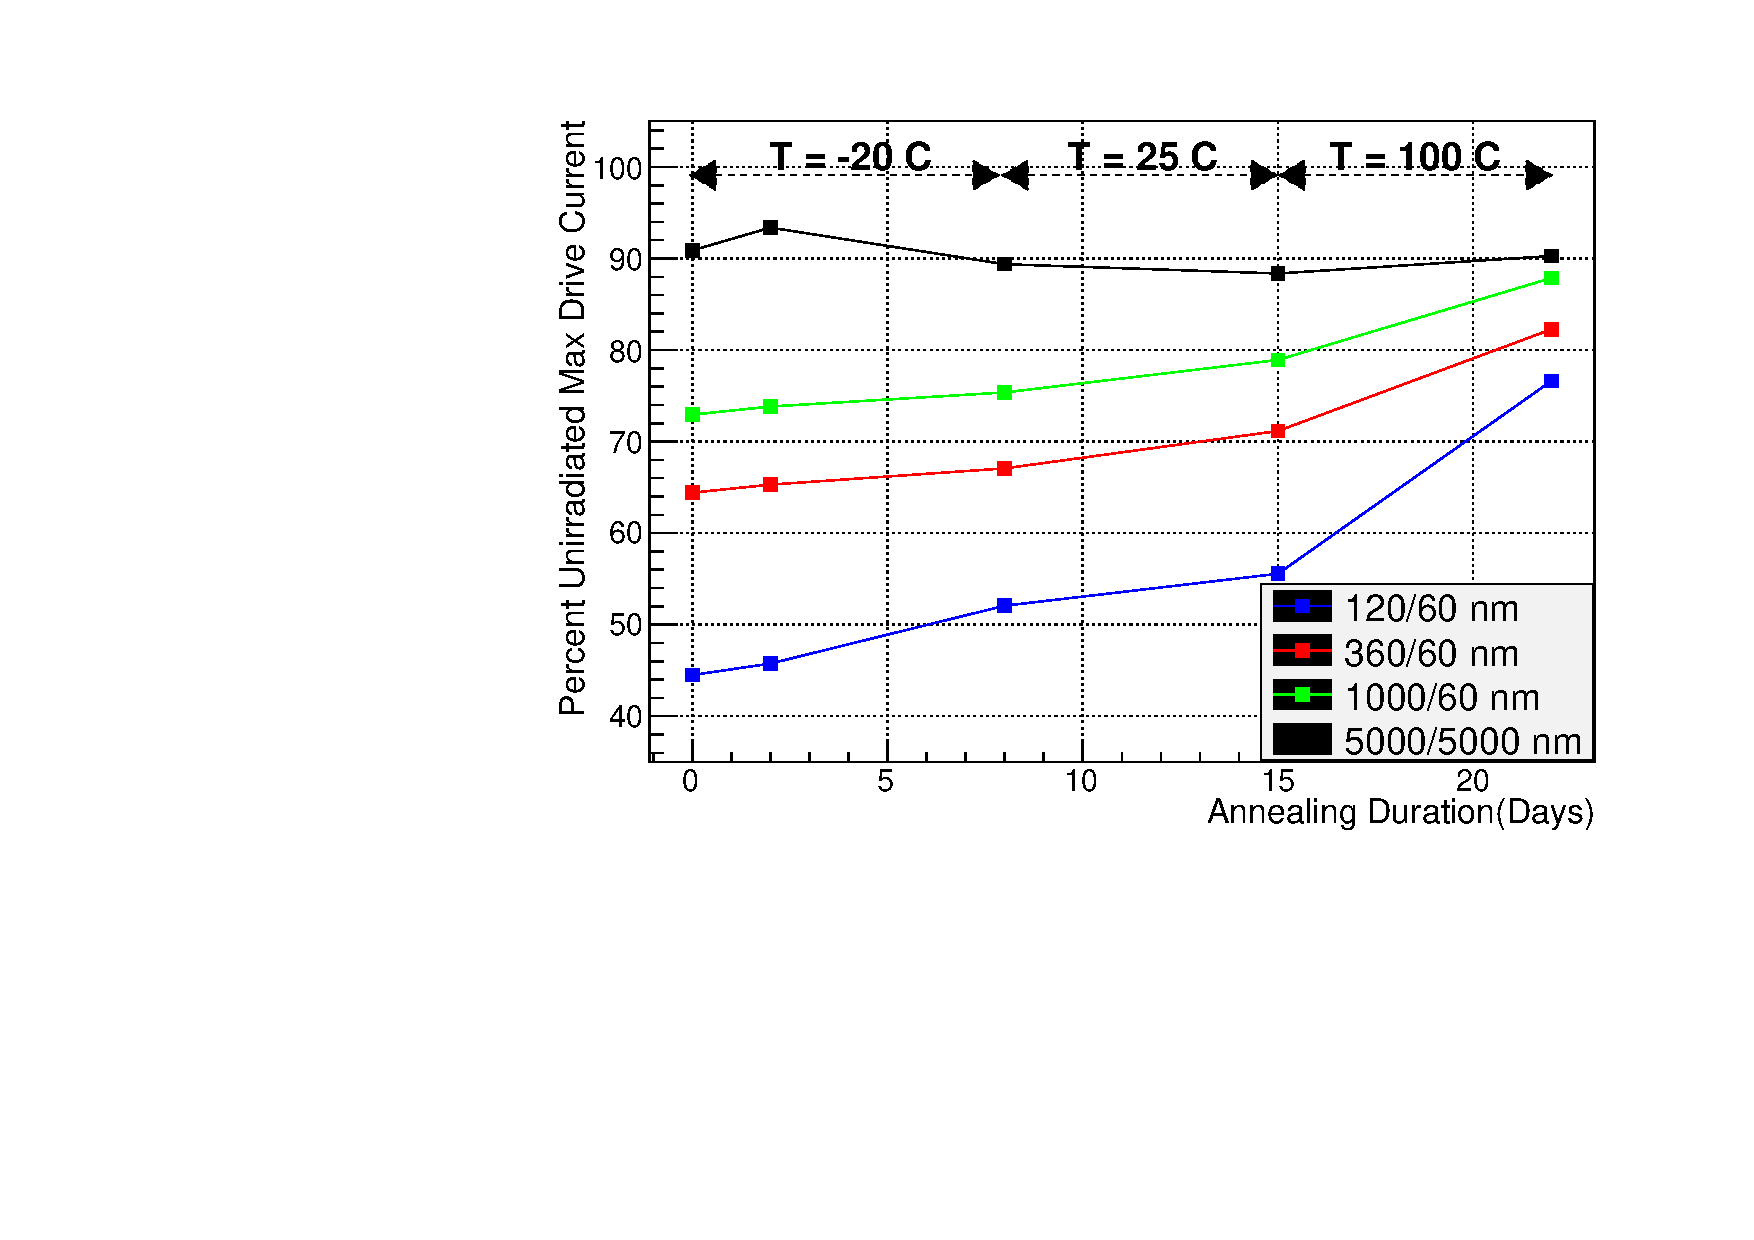
\includegraphics[width=\linewidth]{Comparing_MaxCurDrive_Anneal_PMOS_paper.pdf}
\end{minipage}
\caption{The graph on the left shows the loss of maximum drain-source current during irradiation for 4 PMOS core transistors. The graph on the right shows the recovery of maximum drain-source current for the same 4 transistors during and after annealing.
As in Figure 6, lines are included to make the plots easier to read.
Once again, lines are not drawn through the points corresponding to measurements made after 754 Mrad of transistors in IC5.  The measurements shown for the 5000/5000 transistor are for the transistor in IC7.  For this transistor, no point is included corresponding to an integrated dose of 641 Mrad; we believe that the rotary switch was not set correctly during the measurement of this transistor characteristic since the recorded drain-source current was very small for all values of the gate bias.}
\label{fig:MaxCurDrive_PMOS}
\end{figure}

\begin{figure}
\begin{minipage}[b]{0.5\textwidth}
	\centering
	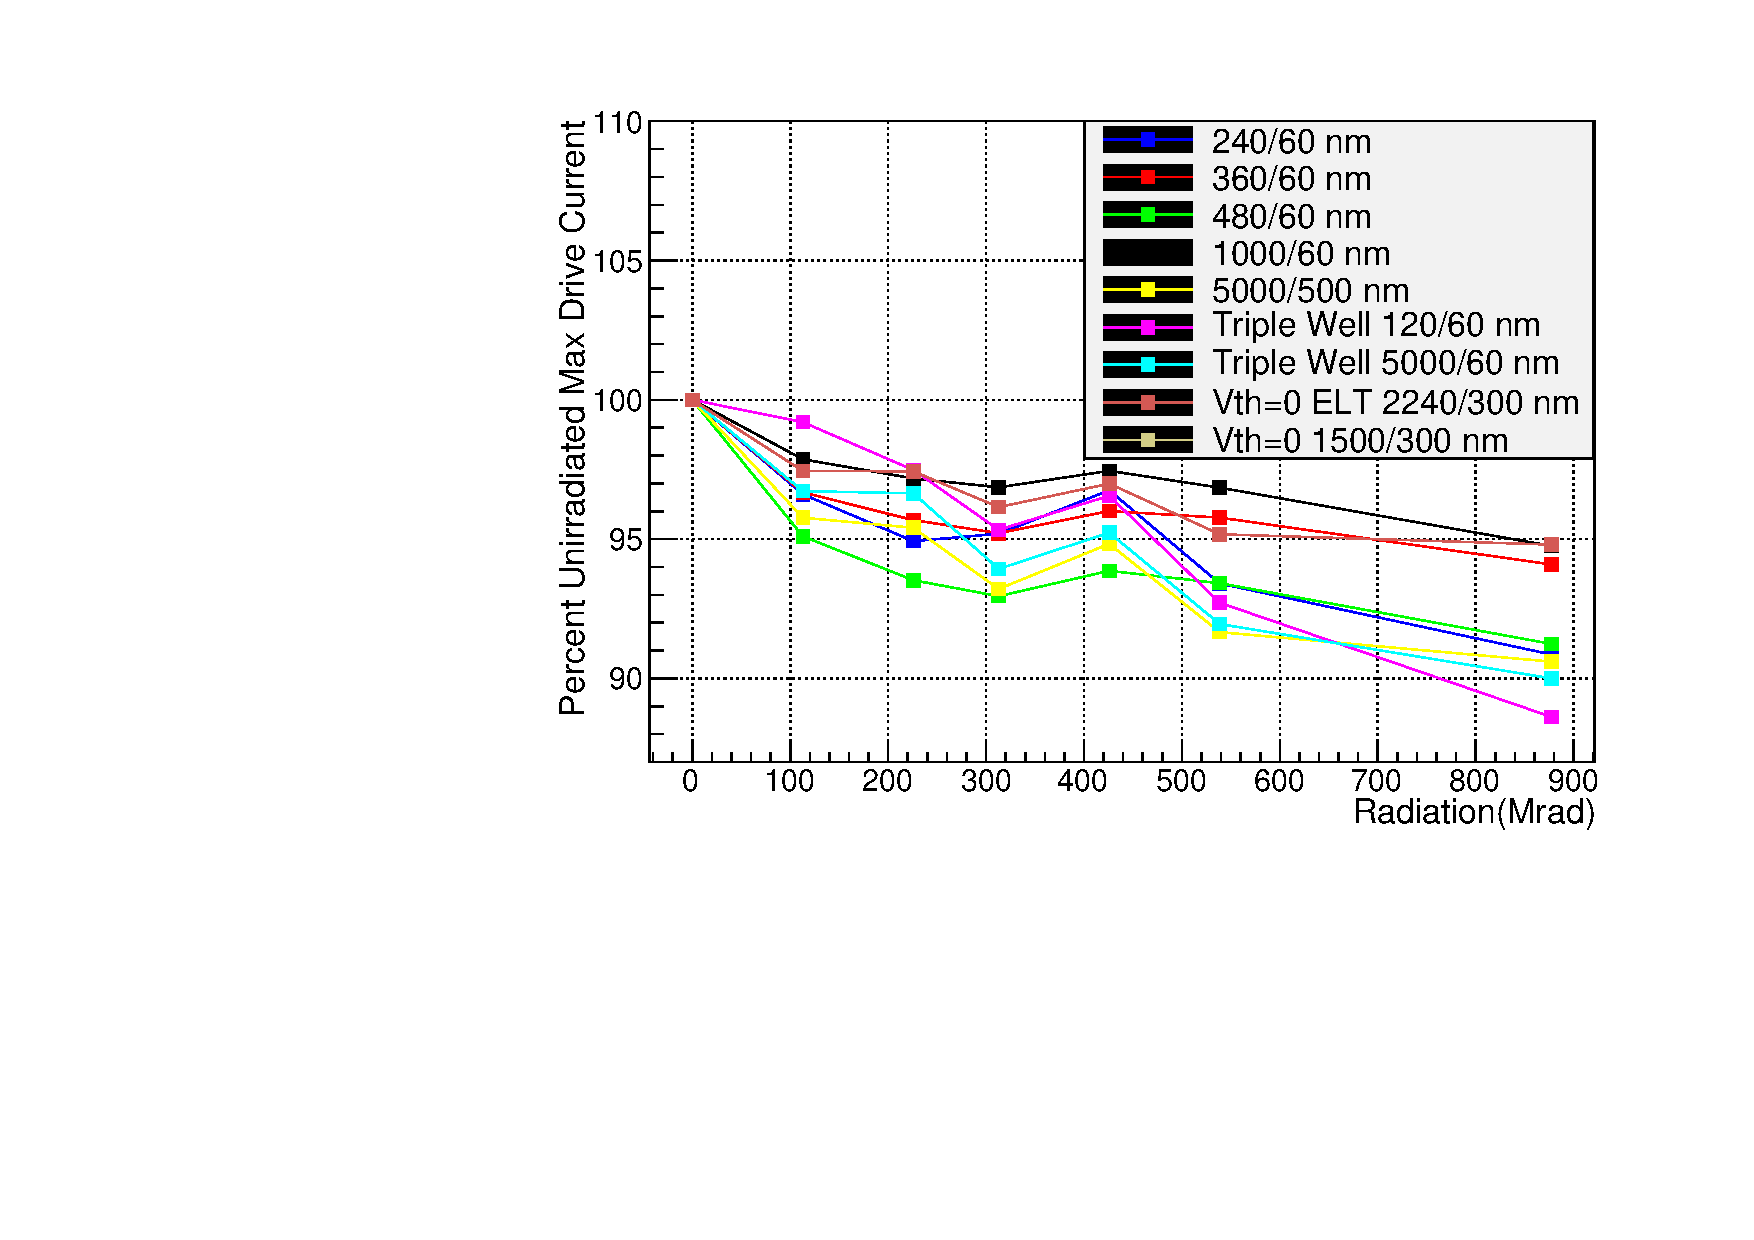
\includegraphics[width=\linewidth]{Comparing_MaxCurrentDrive_NMOS_paper.pdf}
\end{minipage}
\hspace{0.5cm}
\begin{minipage}[b]{0.5\textwidth}
	\centering
	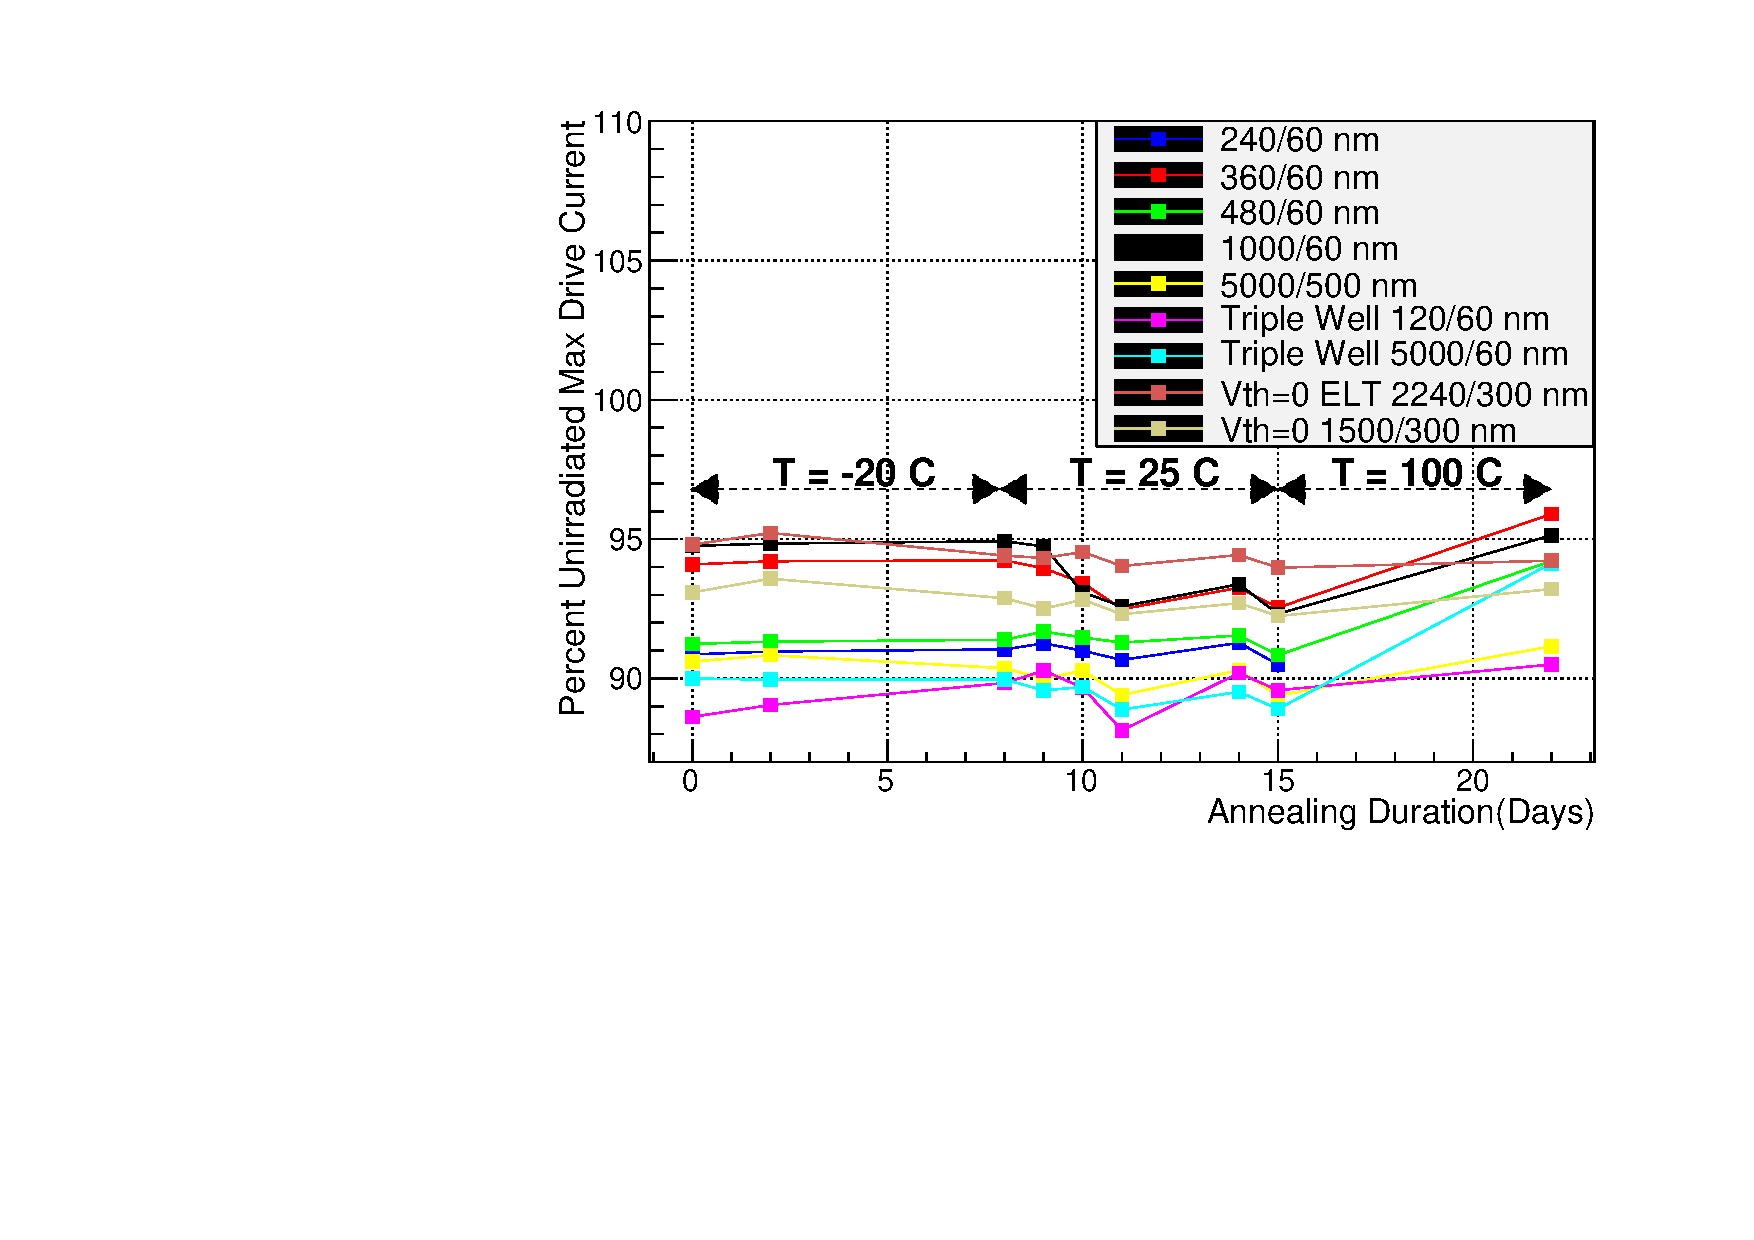
\includegraphics[width=\linewidth]{Comparing_MaxCurDrive_Anneal_NMOS_paper.pdf}
\end{minipage}
\caption{The graph on the left shows the loss in maximum drain-source current after each irradiation step for 9 NMOS core transistors. The graph on the right shows the change in maximum drain-source current for the same 9 transistors during and after annealing.}
\label{fig:MaxCurDrive_NMOS}
\end{figure}

\begin{figure}
\begin{minipage}[b]{0.5\textwidth}
	\centering
	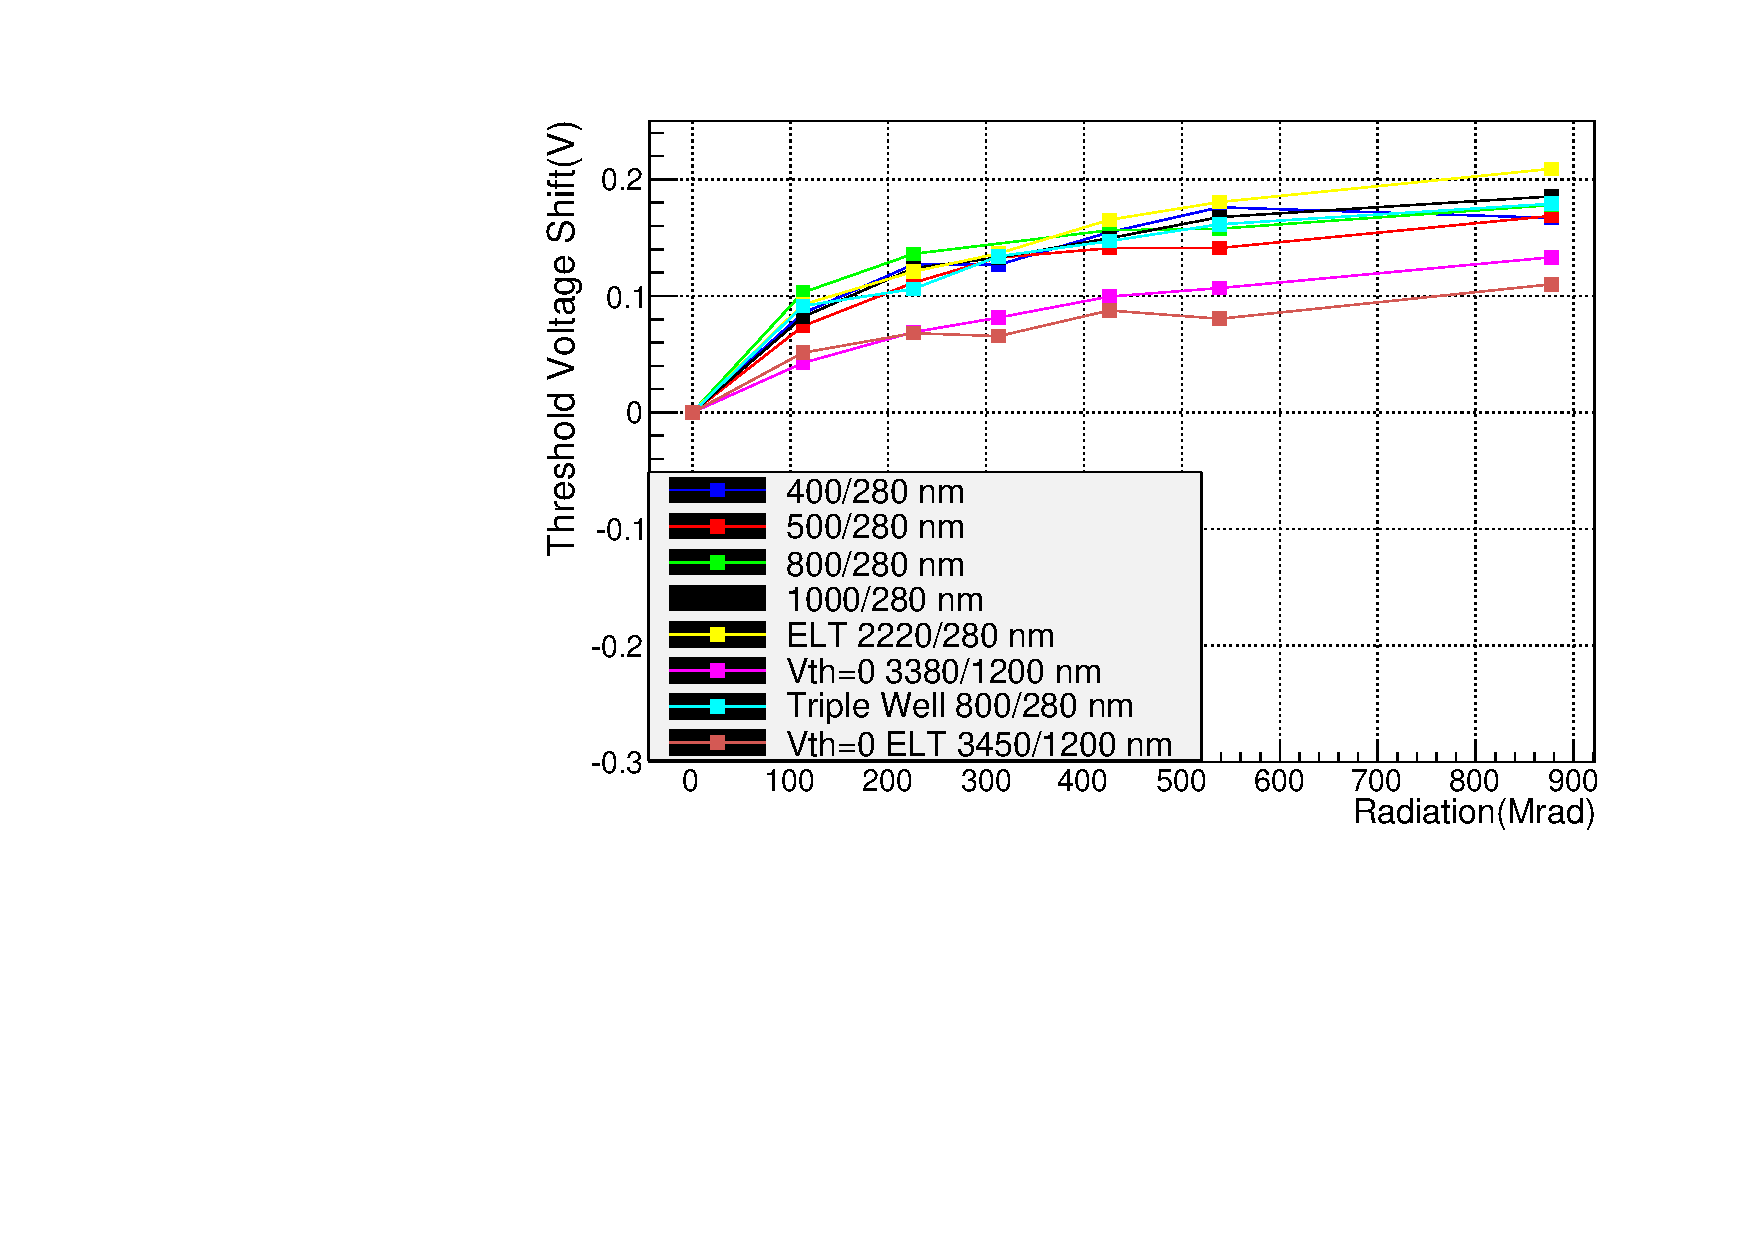
\includegraphics[width=\linewidth]{Comparing_ThreshVolt_DGNMOS_paper.pdf}
\end{minipage}
\hspace{0.5cm}
\begin{minipage}[b]{0.5\textwidth}
	\centering
	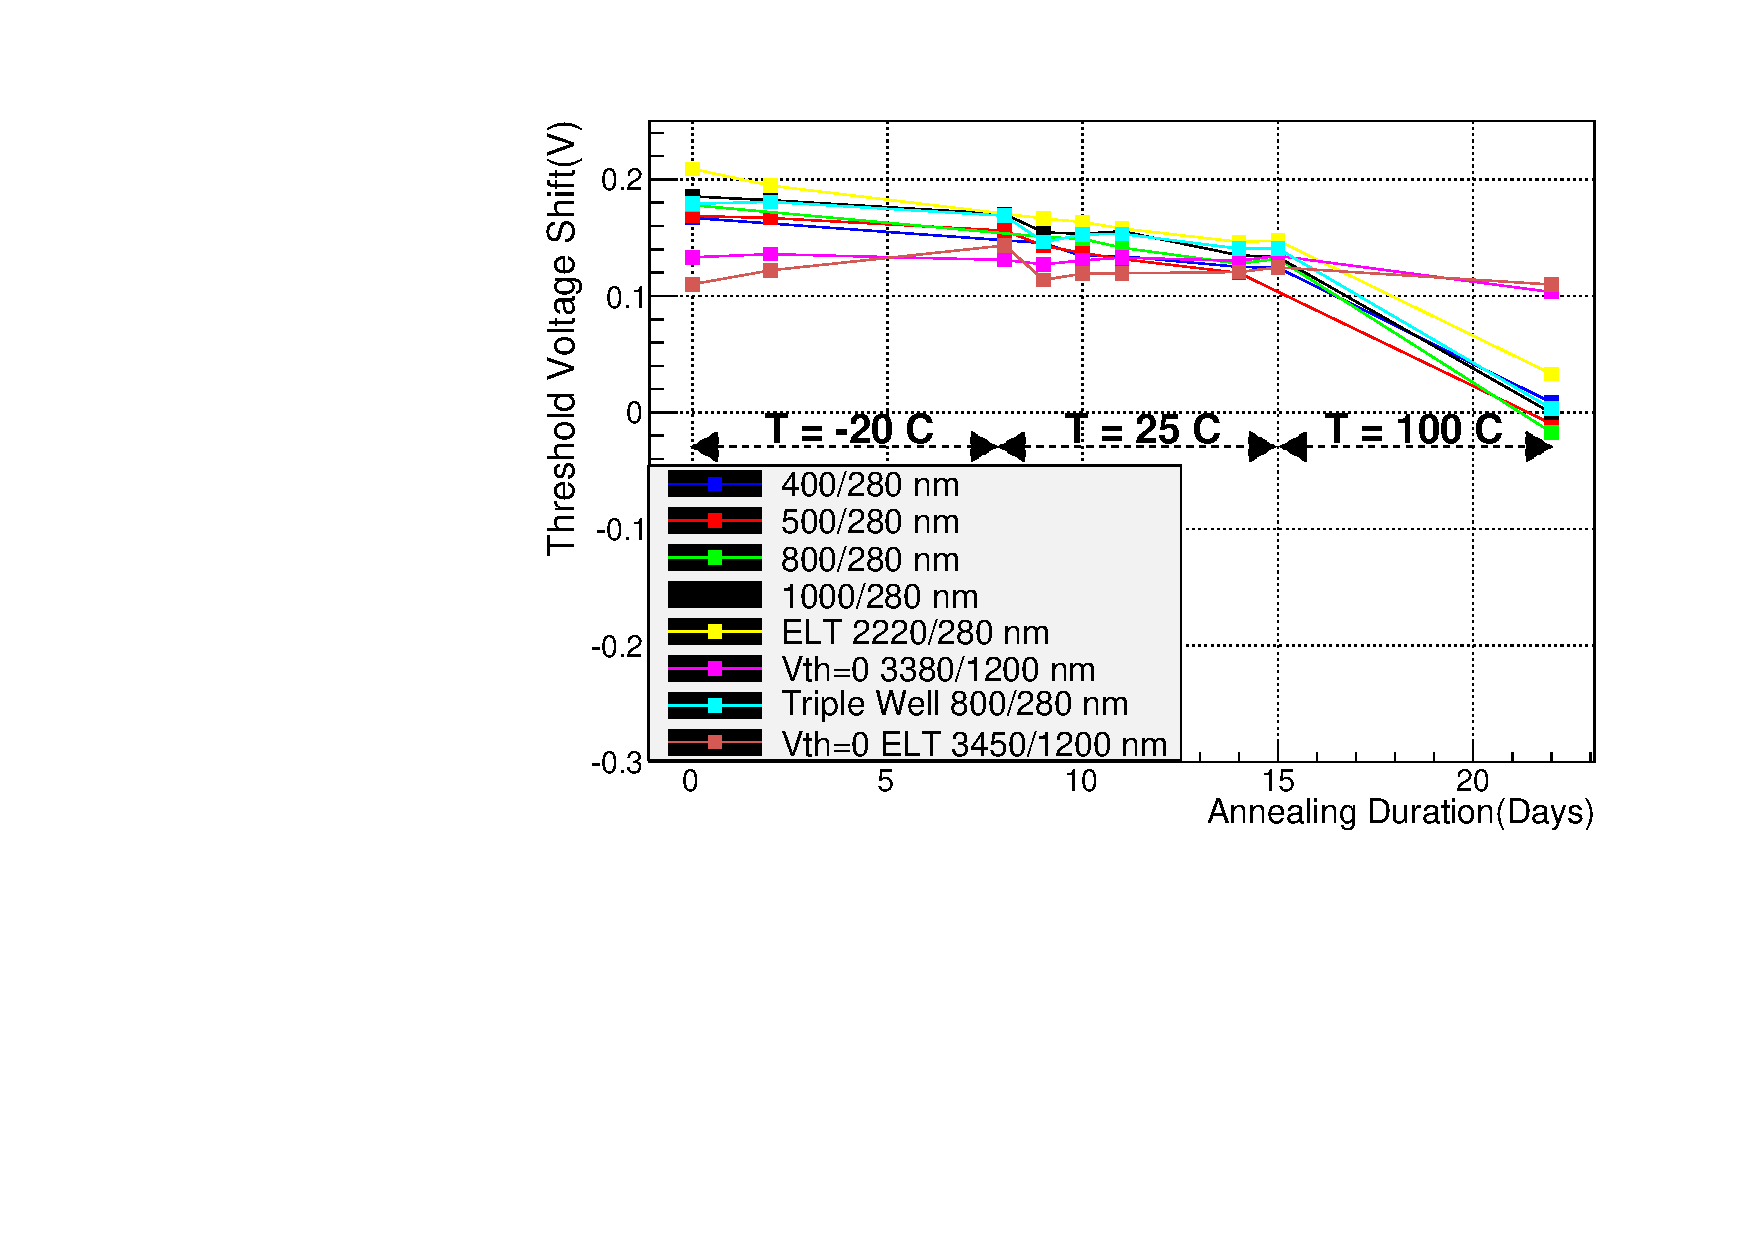
\includegraphics[width=\linewidth]{Comparing_ThreshVolt_Anneal_DGNMOS_paper.pdf}
\end{minipage}
\caption{The shift in threshold voltage for 8 NMOS I/O transistors irradiated to 878 MRad is shown in the graph on the left, while the graph on the right shows $V_{th}$ for the same 8 transistors during and after annealing.  No significant annealing was observed for the two zero $V_{th}$ I/O transistors.}
\label{fig:DGNMOS_Vth}
\end{figure}

Figure~\ref{fig:AnnealSuperpositionPlots} demonstrates the annealing effects observed in our data. Both the PMOS core transistors and the NMOS I/O transistors recovered significantly during the annealing period. 

Figures~\ref{fig:MaxCurDrive_PMOS} and~\ref{fig:MaxCurDrive_NMOS} show the evolution of the maximum drain-source current for a representative selection of PMOS and NMOS core transistors during irradiation and annealing.  We did not observe any significant differences in the effect of radiation on the various different types of NMOS transistors tested (normal layout, enclosed layout, triple well, and zero $V_{th}$).
Figure ~\ref{fig:DGNMOS_Vth} shows the threshold shift of a representative selection of NMOS I/O transistors during irradiation and annealing.
